\documentclass[authoryear,12pt]{article}

\usepackage{amsmath}
\usepackage{amssymb}
\usepackage{xcolor}
\usepackage{graphicx}
%\usepackage{epstopdf}
\usepackage{amssymb}
\usepackage{pifont}
\usepackage{amsmath}
\usepackage{tikz}
\usepackage {longtable} 
\usepackage{tabularx}
\usepackage{natbib}
\usepackage{booktabs}
\usepackage{pdfpages}
\usepackage{epstopdf}
\usepackage{enumerate}

\newcommand{\Rey}{\ensuremath{Re}}
\newcommand{\ord}[1]{\ensuremath{\mathcal{O}(#1)}}
\newcommand{\degree}{\ensuremath{^{\circ}}}

\makeatletter
\newcommand{\rmnum}[1]{\romannumeral #1}
\newcommand{\Rmnum}[1]{\expandafter\@slowromancap\romannumeral #1@}
\makeatother


\newcommand{\ustar}{\ensuremath{U^{*}}}
\newcommand{\mstar}{\ensuremath{m^{*}}}
\newcommand{\cstar}{\ensuremath{c^{*}}}
\newcommand{\reynoldsnumber}{\ensuremath{Re}}
\newcommand{\massstiff}{\ensuremath{\Pi_1}}
\newcommand{\massdamp}{\ensuremath{\Pi_2}}
\newcommand{\ratio}{\ensuremath{\frac{d}{l}}}
\newcommand{\KJ}[1]{{\textcolor{blue}{{\bf{\it{ **KJ: #1 **}}}}}}

\setlength{\textwidth}{180mm}
\setlength{\oddsidemargin}{-10mm}

\begin{document}

\begin{titlepage}
\begin{center}
{\huge \bfseries A study on the energy transfer of a body under fluid-elastic galloping}\\[2.5cm]
{\LARGE \bfseries H.G.K.G Jayatunga}\\[1.5cm]
\Large Supervisors:\\[0.5cm] Dr. Tan Boon Thong \\[0.4cm] Dr. Justin Leontini \\[0.5cm] Dr Huang Yew Mun\\[6.5cm]
\Large Ph.D. Pre-submission seminar\\

\vfill
\textsc{\Large $6^{{th}}$ March 2015}
\end{center}
\end{titlepage}
%\titlepage
%\maketitle
\tableofcontents
\clearpage

\section{Introduction}
\label{sec:intro}
The search for alternative energy sources which could be categorised under the ``green” label has become important area of research in the modern world. Solar, wind power and wave power are some of the examples of these sources. Recently, a new branch of research has been developing to extract energy from flow induced vibrations. It has been hypothesized that this technique may work efficiently in areas where regular turbines cannot.
 
A simple structure that is susceptible to flow-induced vibrations that are suitable for energy extraction are slender structures,such as cylinders, elastically mounted perpendicular to a fluid stream. With regards to a slender body two common types of flow induced vibrations can be observed namely, Vortex Induced Vibrations (VIV) and fluid-elastic galloping. 

The work carried out by \citet{Bernitsas2008a-concept, Bernitsas2009, Raghavan2010a,Lee2011b} and others from the same group at the University of Michigan have made significant progress in finding the possibility of harvesting energy from VIV. However, to this end the possibility of utilising fluid-elastic galloping as a mode of energy harvesting has not been thoroughly investigated. Some theoretical work was carried out by \cite{Barrero-Gil2010a}. What is significant about fluid-elastic galloping is that unlike VIV it is not a resonant type of phenomenon and therefore is not bounded by the narrow range of frequencies which the system has to ``lock-in". Therefore, fluid-elastic galloping may have an advantage over VIV as a potential mode of energy harvesting. 

A weakly non-linear theoretical aeroelastic model to predict the response of galloping was developed by \citet{Parkinson1964} based on a quasi-steady state (QSS) hypothesis. This hypothesis simply claims that only the time-mean lift on the body (averaged over a time much longer than any vortex shedding period) contributes to the dynamics. Lift forces measured experimentally on a static square prism at different angles of attack were used as an input for the theoretical model. This relatively simple model achieved a remarkably good agreement with galloping experiments conducted in a wind tunnel, where the vortex shedding frequency was much higher than the eventual body oscillation frequency, due to the body being relatively heavy.

Most of the literature on galloping using the QSS model has been focused on predicting the displacement amplitude \citep{Parkinson1964,Joly2012,Luo2003}. However, it is quite important to analyse the behaviour of the velocity when studying the power transfer from the fluid to the body. This is because instantaneous power from the fluid flow to the system is the product of the fluid dynamic force and the velocity of the system while instantaneous power out of the system is the product of the damping and the velocity of the system. The fluid dynamic force is also modelled to be only dependent on the velocity of the system. 

The aim of this study is to contribute to the existing knowledge on energy extraction from flow induced vibrations. Hence, investigating the underpinning parameters of the system, the influence of these parameters on energy transfer from the fluid to the body, the relationship of these parameters and the frequency response of the system and investigation  of optimising the energy transfer by controlling the fluid mechanics of the system were the areas of interest.    


\section{Research objectives}

In order to achieve the aim of this study, The three main areas of interest were considered as objectives of this research and therefore, were established as phases of this project. Thus, this project consists of 3 phases. 

\begin{itemize}
\item  Phase 1: understand the underpinning parameters and formulate the appropriate variables of the system.
\item  Phase 2: study the frequency response of the system, and the relationship with the formulated variables.
\item  Phase 3: optimisation of the energy transfer by controlling the fluid mechanics of the system.
\end{itemize}   

\clearpage

\section{Research progress}

\subsection{Phase:1}
 
The focus of this phase was to understand the underpinning parameters of galloping and formulate the appropriate variables to describe the power transfer from fluid to the bodyq. Two non-dimensionalised parameters namely, the combined mass-stiffness (\massstiff) and the combined-mass damping (\massdamp) were formulated using the natural time-scales of the system. The combined mass-damping parameter provided an excellent collapse of mean power and velocity amplitude. This was far better collapse in comparison to the classical Vortex Induced Vibration (VIV) parameters \ustar \ and $\zeta$. The collapse was better than the  More information of the formulation of these parameters and the power and velocity data could be found in appendix 1.    

\subsubsection*{Conclusions}

The following conclusions were made in phase 1 

\begin{itemize}
\item  A good collapse for predicted power output could be obtained by \massstiff \ and \massdamp \ compared to the classical VIV parameters, \ustar and $\zeta$. 

\item The collapsed data using the dimensionless groups shows that the velocity amplitude and the power transfer does not depend on the natural frequency of the system over a large range of frequencies. 

\item In comparison with direct-numerical simulations (DNS) data, it was concluded that the Quasi-steady state (QSS) model (refer appendix 1) provides a good prediction of power output of the system when \massstiff \ is relatively high.   

\item As \massstiff \ is decreased, the deviation between QSS and DNS data increases as the influence of vortex shedding becomes more stronger.   
\end{itemize}

\clearpage
\subsection{Phase:2}
 
 The formulation of \massstiff \ and \massdamp \ lead to investigating the impact of these variables on the frequency of the system. The eigenvalues of the system were expressed using \massstiff \ and \massdamp (refer equation 5 appendix 2). While the eigenvalues remain complex, (the term under the square root remains negative) the imaginary component could be defined as the frequency of the system. Since this frequency was obtained using the linearised QSS equation, it could be identified as the linear predicted frequency. However, for a given \massdamp \ value, there is a limit of \massstiff \ below which the eigenvalues becomes real or the square root term positive. Therefore a linear predicted frequency does not exist. However, the QSS model produces a signal and therefore a frequency is present in this region. This is because non linear terms in the forcing function become dominant.
 
 \subsubsection*{Conclusions}

\begin{itemize}

\item The linear frequency of the system could be obtained form the imaginary component of the eigenvalue equation of the linearised QSS model, (refer equation 5 appendix 2) provided that the square root term remains complex. 

\item This equation provides a good prediction of the frequency at high \massstiff. However, it deviates as \massstiff \ reduces because the non linear terms start to dominate the forcing. 

\item The linearised equation fails to predict the frequency at the point where the term under the square root positive. However, the general QSS model does output a frequency.  

\item The region where the linear expression of frequency fail could not be captured in the DNS data, as the vortex shedding becomes stronger and therefore suppresses galloping. 


\end{itemize}

\clearpage

\subsection{Phase:3}

This phase was focused on analysing the fluid dynamics involved in galloping and how it can be manipulated to get an optimum power output. With existing literature it was clear that the induced lift on a galloping body will increase until it reaches the shear layer re-attachment. Therefore, it was hypothesised that delaying the re attachment of the shear layer could lead to effective higher power output. In order to do this, the afterbody of the square cross section was tapered away. (figure \ref{fig:hybrid_section}). The tapering was carried out incrementally by changing $\frac{d}{l}$ ratio. Four cross sections were obtained at $\frac{d}{l}= 0.75,0.5,0.25 \ \text{and} \ 0$. Figure \ref{fig:lift_curves} shows the stationary lift data at different angle of attack. 

 \vspace{30mm}
\begin{figure}
\setlength{\unitlength}{\textwidth}

  \begin{picture}(1,0.23)(0,0.74)
    
  \put(0.2,0.76){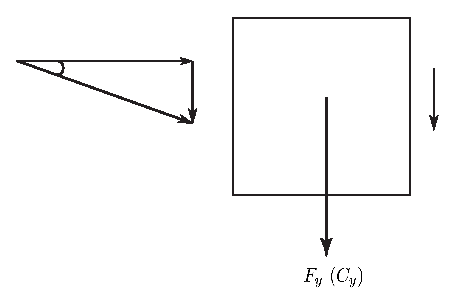
\includegraphics[width=0.5\unitlength]{../FnP/gnuplot/setup-1.eps}}         
      
      
   
 	\put(0.315,0.93){$U$}
 	\put(0.3,0.84){$U_i$}
    \put(0.42,0.88){$\dot{y}$}
    \put(0.28,0.895){ $\theta$}
    \put(0.7,0.87){\small $(+)$}
      	

 	
 	 

     

  \end{picture}

 \caption{Induced angle of attack on the square prism due to the resultant of free-stream velocity of the fluid and transverse velocity of the body.}
    \label{fig:setup_1}
\end{figure}

\begin{figure}
  \setlength{\unitlength}{\textwidth}

  \begin{picture}(1,0.75)(0,0)
    % % %90
      % % % Parkinson Data 
      \put(0.035,0.5){\includegraphics[width=0.5\unitlength]{./FnP/lift_curve_sq.eps}}
      \put(0.495,0.5){\includegraphics[width=0.5\unitlength]{./FnP/lift_curve_075.eps}}
      \put(0.035,0.27){\includegraphics[width=0.5\unitlength]{./FnP/lift_curve_05.eps}}
      \put(0.495,0.27){\includegraphics[width=0.5\unitlength]{./FnP/lift_curve_025.eps}}
      \put(0.3,0.0){\includegraphics[width=0.5\unitlength]{./FnP/lift_curve_tri.eps}}
      
      
   
      
      
%      \put(0.23,0.00){ $\displaystyle\frac{c}{\rho\mathcal{A}U}$}
%      \put(0.73,0.00){ $\displaystyle\frac{c}{\rho\mathcal{A}U}$}

      \put(0.3,0.26){$\theta$}
      \put(0.76,0.26){$\theta$}
      \put(0.56,-0.01){$\theta$}
      
      \put(0.01,0.405){$\displaystyle C_y$}
       \put(0.01,0.65){$\displaystyle C_y$}
      \put(0.3,0.14){$\displaystyle C_y$}
      
      \put(0.106,0.705){\small(a)}
      \put(0.565,0.705){\small(b)}
      \put(0.106,0.475){\small(c)}
      \put(0.565,0.475){\small(d)}
      \put(0.37,0.207){\small(e)}
      

  \end{picture}

  \caption{Induced lift coefficient $C_y$ at different angles for selected cross sections. Data presented for cross sections, (a) square, (b) $\ratio=0.75$, (c) $\ratio=0.5$, (d) $\ratio=0.25$ and (e) triangle.}
  \label{fig:lift_curves}
\end{figure}




\subsection{Preliminary conclusions}





\clearpage

\section{Structure of the thesis}

\begin{enumerate}
	
	\item Preliminary remarks 
	\item A review of literature
		\begin{enumerate}[i]
		\item Introduction
		\item Flow induced vibrations 
		\item Flow induced vibrations and energy harvesting
		\item Fluid-elastic galloping
		\item Induced lift and the influence of the shear layers 
	\end{enumerate}
	\item Methodology and validation
	\begin{enumerate}[i]
		\item Introduction
		\item Governing equations and quasi-steady state model 
		\item Numerical methods and boundary conditions 
		\item The governing equations for the DNS method: Naiver-Stokes and continuity
		\item Convergence and validation studies 
		\item Summary
	\end{enumerate}	
	\item Governing parameters of  fluid-elastic galloping
	\begin{enumerate}[i]
		\item Introduction 
		\item Static body results 
		\item Formulation of the non-dimensionalised parameters \massstiff \ and \massdamp 
		\item Comparison of \massstiff \ and \massdamp \ with classical VIV parameters
		\item Comparison of power between high and low \reynoldsnumber\ data
		\item Dependence on the mass ratio \mstar
		\item Summary 
	\end{enumerate}	
	\item Frequency response of the system
	\begin{enumerate}[i]
		\item Introduction 
		\item Prediction of linear frequency 
		\item QSS and DNS frequency data 
		\item Comparison of linear frequency data with QSS and DNS data
		\item Summary 
	\end{enumerate}		
	\item Optimisation of the cross sectional shape 
	\begin{enumerate}[i]
		\item Introduction 
		\item Stationary data 
		\item Mean power data 
		\item Time average data 
		\item Flow characteristics. 
		\item FSI validation
		\item Summary 
	\end{enumerate}
	
\end{enumerate}

\clearpage
%\section{Revised gantt chart}
%\begin{figure}[h!]
%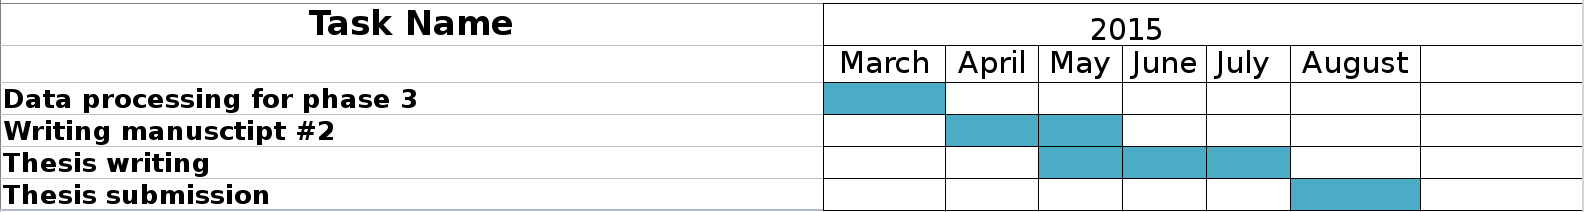
\includegraphics[width=1\linewidth]{./gantt}
%\caption{Revised gantt chart}
%\label{fig:gantt}
%\end{figure}




\clearpage
\bibliographystyle{elsarticle-harv}
\bibliography{Paper.bib}

\clearpage
\section*{\LARGE Appendix 1}
\label{app:manuscript}
\addcontentsline{toc}{section}{Appendix 1}
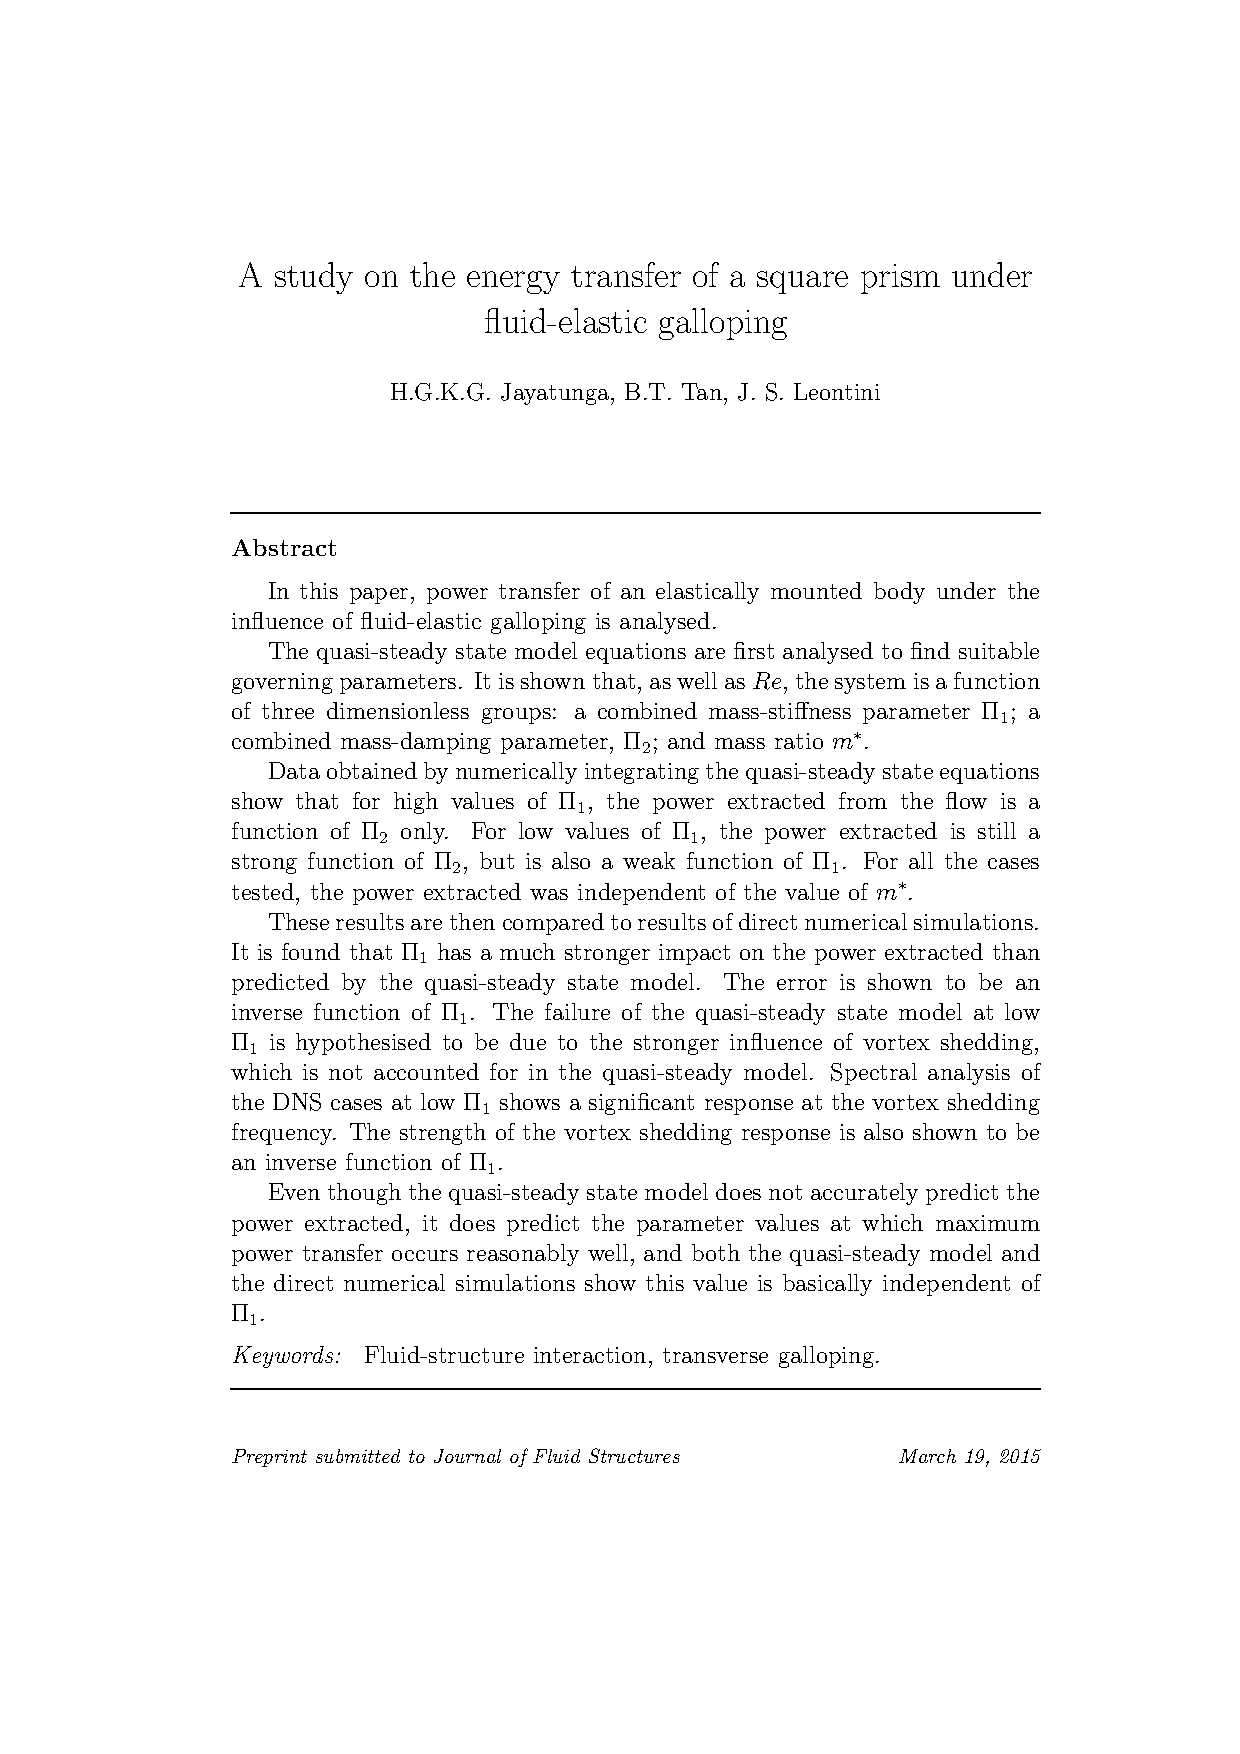
\includepdf[pages=1-30]{elsarticle-template-harv.pdf}

\clearpage
\section*{\LARGE Appendix 2}
\addcontentsline{toc}{section}{Appendix 2}
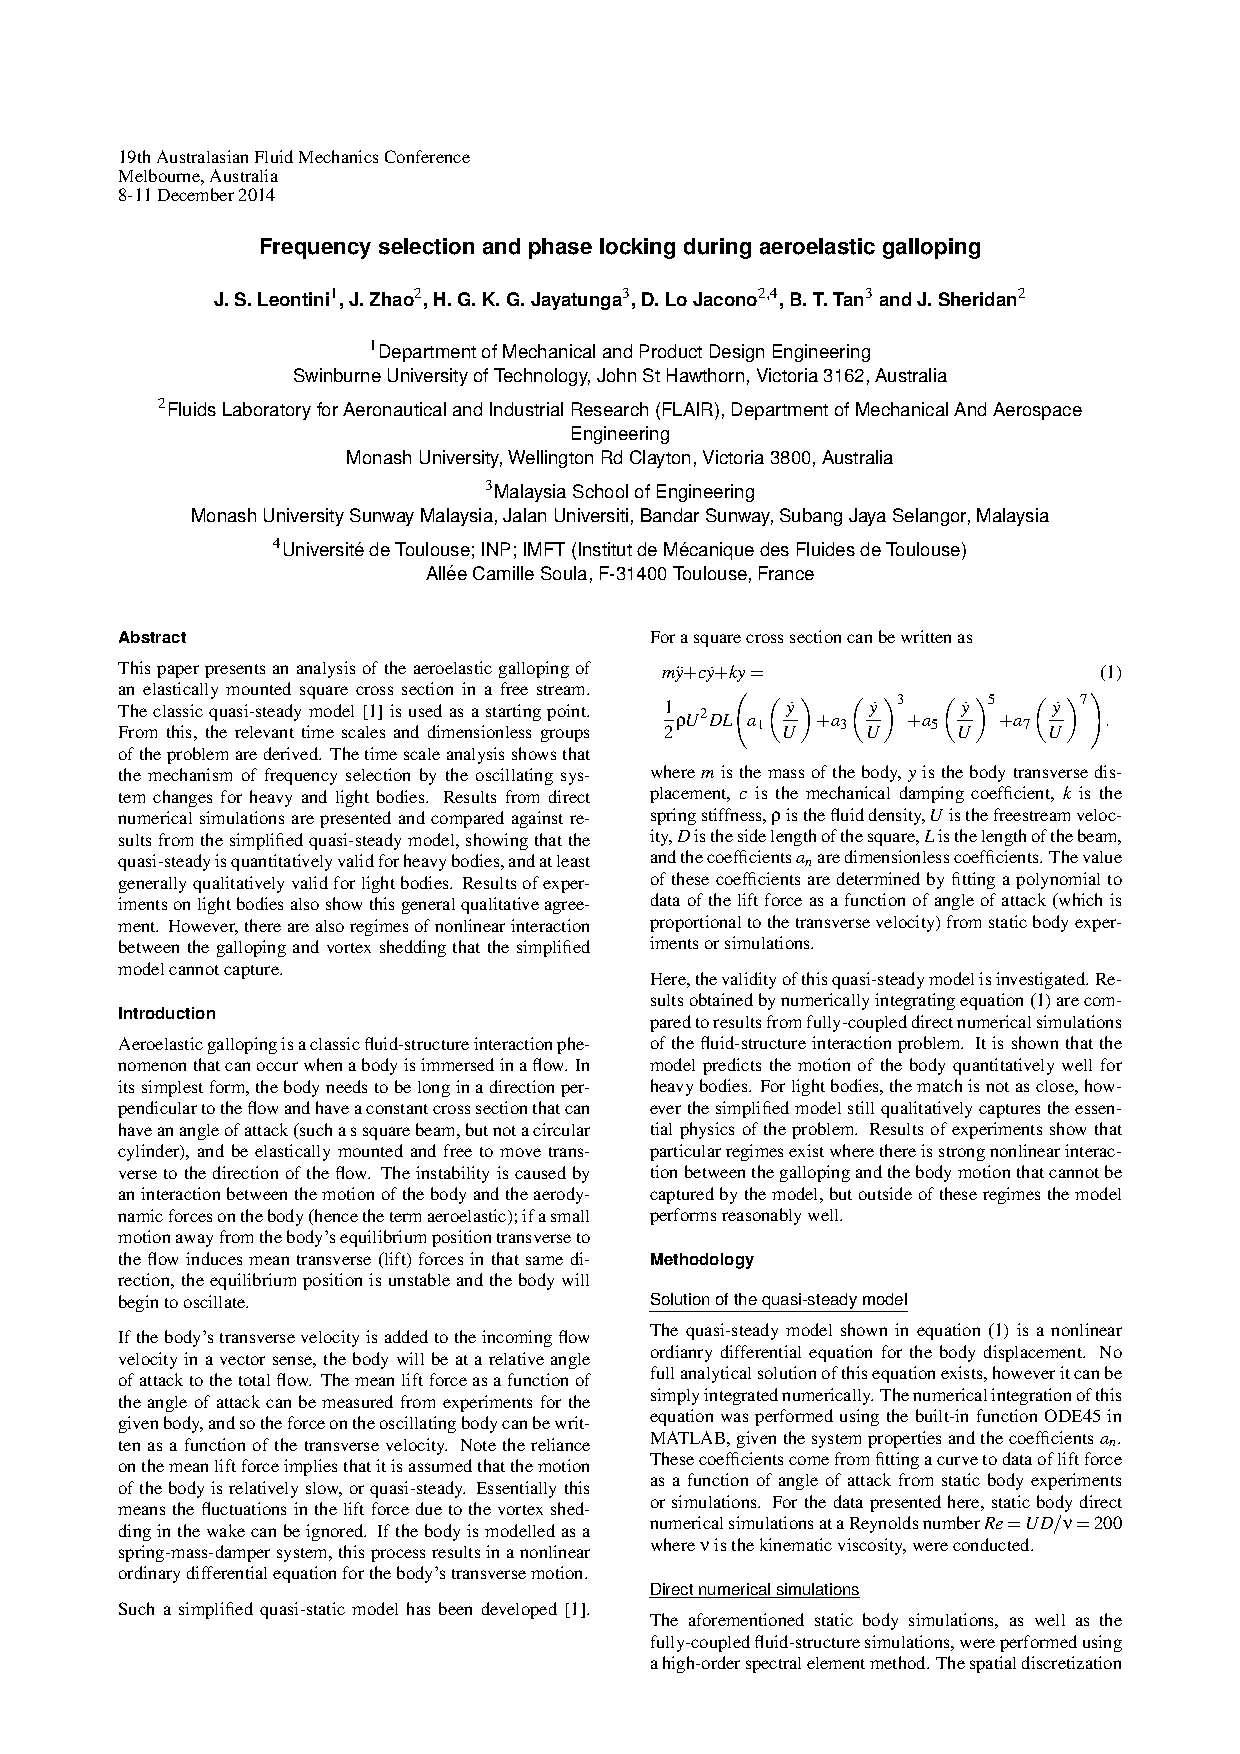
\includepdf[pages=1-4]{galloping_paper.pdf}
\end{document}








